

\section{Problem 2}
\label{part2}
\begin{verbatim}

Download the TimeMaps for each of the target URIs.  We'll use the mementoweb.org 
Aggregator, so for example:

URI-R = http://www.cs.odu.edu/

URI-T = http://mementoweb.org/timemap/link/http://www.cs.odu.edu/

You could use the cs.odu.edu aggregator:

URI-T = http://mementoproxy.cs.odu.edu/aggr/timemap/link/1/http://www.cs.odu.edu/

But be sure to say which aggregator you use -- they are likely to give
different answers.

Create a histogram of URIs vs. number of Mementos (as computed from
the TimeMaps).  For example, 100 URIs with 0 Mementos, 300 URIs
with 1 Memento, 400 URIs with 2 Mementos, etc.

See: http://en.wikipedia.org/wiki/Histogram

Note that the TimeMaps can span multiple pages.  Look for links like:

<http://mementoweb.org/timemap/link/1000/http://www.cnn.com/>;rel="timemap"; 
type="application/link-format"; from ="Sun, 08 Jul 2001 21:30:54 GMT"

This indicates another page of the TimeMap is available.  There can be 
many pages to a TimeMap.
\end{verbatim}

\subsection{Solution}
\begin{enumerate}
\item In order to compute the mementos for a link we need the TimeMap for each link from the file containing many links which is an out from the first question.
\item I used "http://mementoweb.org/timemap/link/" because it worked better than http://mementoproxy.cs.odu.edu/aggr/timemap/link/1.And the mementoproxy provided cs department was very slow.   
\item After finding the Time Map for each link parse them and count the mementos.
\item When the request that generate a 404 are recorded as having 0 mementos.and these mementos are counted using a regular expression.
\item I have written Two functions named getTimeMap\(url\) which get the timemaps for each link provided and countMementos\(mem\_url\) which counts the mementos for each timemap generated by the other function. 
\item There can be many pages to a TimeMap.so written a while loop which checks for any timemaps which directs to an other page and found the total count of mementos

\item Finally extracting the mementos and the url name.  
  
\end{enumerate}
\newpage
\subsection{Code Listing}
\subsubsection{mementocount.py}
\lstinputlisting[language=Python,breaklines = true,frame=single,caption={Python program for counting mementos}, label=lst:q1-1,captionpos=b,numbers=left,showspaces=false,showstringspaces=false,basicstyle=\footnotesize]{mementocount.py}
\newpage
\subsubsection{histogram.R}
\lstinputlisting[language=R,breaklines = true,frame=single,caption={R program for generating the histograms for Question 2}, label=lst:q2R,captionpos=b,numbers=left,showspaces=false,showstringspaces=false,basicstyle=\footnotesize]{histogram.R}
\begin{enumerate}
\item Initial I created a histogram with the output i got from the countmementos.py but the graph looked like in the Figure 1 in page 15
\item There is  
\item There are 500 links with 0 mementos and 90 links with more than 1000 mementos and 59 links with 1 memento and 30 links with 2 and other links have mementos mostly under 500. which means majority of the links fall under 1000 mementos. 
\item When plotted the histogram for the above data we get Figure 1 which does not give any proper visualization 
\item I am not satisfied with the figure 1, so i made few changes in order get a decent histogram.
\item So i stripped out the mementos which are grater than 1000 as there are only 90 so this data gives Figure 2 in page 10 which seems little better than the previous one
\item  If we focus more on the highest number of records,mementos less than 200 then the plot actually begins to look more like a histogram in Figure in page 11 
\end{enumerate}

\newpage
\subsection{Results}
\subsubsection{Output for the mementocount.py}
\verbatiminput{samplemementos.txt}
\newpage
\subsubsection{Histograms}
\begin{figure}[ht]    
    \begin{center}
        
\includegraphics[scale=0.60]{q2-histogram1.png}
        \caption{Histogram 1}
        \label{Histogram 1}
    \end{center}
\end{figure}
\newpage
\begin{figure}[ht]    
    \begin{center}
        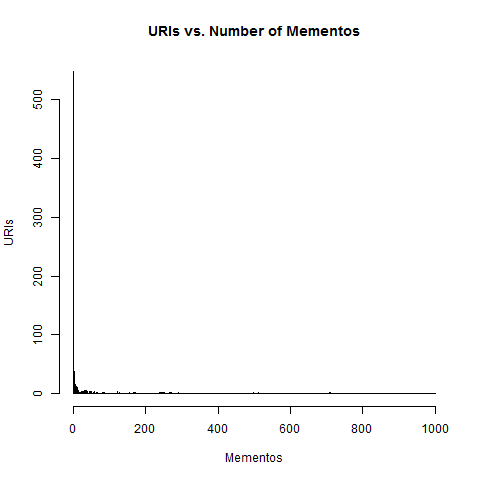
\includegraphics[scale=0.60]{q2-histogram2.png}
        \caption{Histogram 2}
        \label{Histogram 2}
    \end{center}
\end{figure}
\newpage
\begin{figure}[ht]    
    \begin{center}
        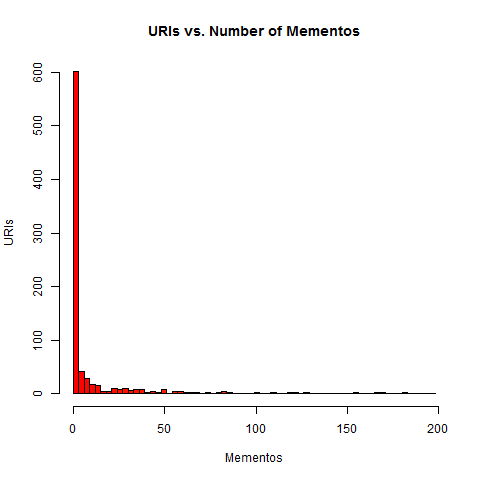
\includegraphics[scale=0.60]{q2-histogram3.png}
        \caption{Histogram 3}
        \label{Histogram 3}
    \end{center}
\end{figure}
\newpage